\subsection*{Wi-Fi Physical Layer}
The further development of IEEE 802.11 is accompanied by a constant change of the physical layer. \textcite{sauter_wireless_2022} mentions, that all new enhancements of the physical layer of IEEE 802.11 are backward compatible to previous definitions of the it.

According to the Author, IEEE 802.11 initially used DSSS and FHSS as modulation methods.
Since IEEE 802.11g the modulation method \ac{OFDM} can be used in the \SI{2.4}{\giga\hertz} frequency band. the author explains \ac{OFDM} as following. \ac{OFDM} divides the transmission channel in subcarriers with different amplitudes, frequencies and phases. Each subcarrier is orthogonal to another one, as they send the information "Low", where only one other subcarrier is sending the information "High". 

\subsubsection*{Symbol length}
The data is then sent as \ac{OFDM} symbols over the individual \ac{OFDM} subcarriers. The distance between the "highs" of the subcarriers is specified as subcarrier spacing and corresponds to the reciprocal symbol length. This has now increased from \SI{3.2}{\micro\second} for IEEE 802.11n to \SI{12.8}{\micro\second} for IEEE 802.11ax. This corresponds to a subcarrier spacing of \SI{312.5}{\kilo\hertz} and \SI{78.125}{\kilo\hertz} respectively. 

For the IEEE 802.11p and IEEE 802.11bd standards, a symbol length of \SI{6.4}{\micro\second} applies, corresponding to a subcarrier spacing of \SI{156.25}{\kilo\hertz} \cite{jacob_system-level_2020}.

For the modulation and demodulation of the transmitting bits the FFT and IFFT are used respectively. With the reduction of the subcarrier spacing, more subcarriers are created in the transmission channel, so that the FFT size must be increased. 

\textcite{kauffels_wireless_2002} adds, that \ac{OFDM} can be used in the \SI{5}{\giga\hertz} frequency band since IEEE 802.11a. 
\subsubsection*{\acf{BW}}
\subsubsection*{\acf{MCS}}

In order to encode as many bits as possible on one \ac{OFDM} symbol, different \ac{MCS}s can be used.   
These \ac{MCS}s for the IEEE 802.11 standards are based on \ac{PSK} or \ac{QAM}. \cite{kauffels_wireless_2002}. 
The smallest \ac{MCS} is binary \ac{PSK} and encodes \SI{1}{\bit} per symbol. IEEE 802.11ax has the most complex \ac{MCS} of \num{256}-\ac{QAM} IEEE 802.11ac to \num{1024}-\ac{QAM} and thus now encodes \SI{10}{\bit} per symbol \cite{afaqui_ieee_2017}.
In the \ac{V2X} range, so can \ac{MCS}s from binary-\ac{PSK} to \num{256}-\ac{QAM}.

In order to encode as many bits as possible on one \ac{OFDM} symbol, different \ac{MCS}s can be used.   
The \ac{MCS}s for the IEEE 802.11 standards are based on \ac{PSK} or \ac{QAM}. \cite{kauffels_wireless_2002}. 
The smallest \ac{MCS} is Binary - \ac{PSK} and encodes \SI{1}{\bit} per symbol. IEEE 802.11ax has the most complex \ac{MCS} of \num{256} - \ac{QAM} IEEE 802.11ac to \num{1024} - \ac{QAM} and thus now encodes \SI{10}{\bit} per symbol \cite{afaqui_ieee_2017}.
In the \ac{V2X} range, so can \ac{MCS}s from binary-\ac{PSK} to \num{256}- \ac{QAM}.

An imaginary, theoretical transmission channel is usually specified as a square-wave signal in the frequency domain with the limits of both minimum and maximum amplitude and cut-off frequency. \textcite{kauffels_wireless_2002} defines the roll-off factor as a cosine-shaped flattening of the square signal between 0 and 1. In addition, the author points out that \ac{QAM} can generate high roll-off factors, so that signals interfere significantly more with adjacent channels.

In this regards the author recommends setting the parameters in an \ac{OFDM} system in such a way that first the coding rate and then the complexity of the \ac{MCS} is reduced in difficult transmission environments. The more bits a \ac{MCS} encodes on a symbol, the more error-prone the correct decoding of the symbol.

\subsubsection*{\acf{FEC}}

Nevertheless bit errors can occur during the transmission. In this regard, \cite{kauffels_wireless_2002} mentions and explains \ac{FEC} as a technique to reduce bit errors during transmission. \ac{FEC} adds redundant bits to the data. The receiver uses these redundant bits to check the integrity or correct errors of the received data. The proportion of non-redundant transmission bits is defined in \ac{CR} \todo{explain cr ?? Cite??}

To achieve this, \ac{BCC} is used mandatory since the IEEE 802.11n standard \cite{afaqui_ieee_2017} \cite{syafei_performance_2009}. \textcite{syafei_performance_2009} add that it is optionally possible to use \ac{LDPC}. The authors state that \ac{LDPC} can achieve a better channel capacity performance. This is also confirmed by \textcite{afaqui_ieee_2017}, who point out that \ac{LDPC} also generates higher computational cost. 

IEEE 802.11ax stations must support \ac{LDPC} when using on the IEEE 802.11ax standard under the following conditions \cite{afaqui_ieee_2017} \cite{noauthor_ieee_2021}:
\begin{itemize}
	\item The used bandwidth is greater than \SI{20}{\mega\hertz}
	\item The chosen \ac{MCS} is \num{1024}-\ac{QAM}
	\item More then four transmission channels are used for the transmission. 
\end{itemize}
IEEE 802.11ax achieves \ac{CR} of \nicefrac{1}{2}, \nicefrac{2}{3}, \nicefrac{3}{4}, and \nicefrac{5}{6} \cite{noauthor_ieee_2021}.
Similarly, IEEE 802.11p uses the \ac{BCC} technique, which has been superseded by \ac{LDPC} in its successor IEEE 802.11ax \cite{jacob_system-level_2020} \cite{krief_analysis_2020}. \textcite{krief_analysis_2020} argue that this step was important, as \ac{LDPC} offers better error correction possibilities for higher communication ranges greater than \SI{50}{\metre}.

Together with the \ac{MCS}, the \ac{FEC} \ac{CR} form a physical layer specification. This is named after the standard and includes the possible expressions for \ac{MCS} values and \ac{CR} of the standard. For IEEE 802.11ax, this results in the HE-MCS index values in \autoref{tab:HEMCS}

\begin{table}[!ht]
	\centering
	\begin{tabular}{>{\raggedright}p{2cm}p{3cm}p{2cm}}
		\toprule
		HE-MCS index & \acf{MCS} & \acf{CR} \\
		\midrule
		\num{0} & Binary \ac{PSK}& \nicefrac{1}{2}\\
		1 &  Quadrature \ac{PSK}& \nicefrac{1}{2}\\
		2 &  Quadrature \ac{PSK}& \nicefrac{3}{4}\\
		3 &  \num{16}-\ac{QAM}& \nicefrac{1}{2}\\
		4 &  \num{16}-\ac{QAM}& \nicefrac{3}{4}\\
		5 &  \num{64}-\ac{QAM}& \nicefrac{2}{3}\\
		6 &  \num{64}-\ac{QAM}& \nicefrac{3}{4}\\
		7 &  \num{64}-\ac{QAM}& \nicefrac{5}{6}\\
		8 &  \num{256}-\ac{QAM}& \nicefrac{3}{4}\\
		9 &  \num{256}-\ac{QAM}& \nicefrac{5}{6}\\
		10 &  \num{1024}-\ac{QAM}& \nicefrac{3}{4}\\
		11 &  \num{1024}-\ac{QAM}& \nicefrac{5}{6}\\
		\bottomrule
	\end{tabular}
	\caption{HE-\ac{MCS} index table nach \cite{noauthor_ieee_2021}}
	\label{tab:HEMCS}
\end{table}


\todo{Symbol length, GI, subcarrier spacing reciprocal}
\todo{Wellenausbreitung, Überlagerungseffekte, Reflexsion, Reflexsion nicht bei Metall}
\todo{Knauffel OFDM PHY}

\subsubsection*{\acf{GI}}
\textcite{pulimamidi_development_2007} explain the Guard Interval as a cyclic prefix of OFDM symbols before Inter Symbol Interference and through Inter Carrier Intereference. Inter Symbol Interference is caused by multipath delays , where the reflected delayed previous symbol can interfere with the current received symbol\cite{ravindranath_performance_2016}. Similarly, Inter Carrier Interference is caused by time-varying channel a longer OFDM symbol duration, that just as an interference with the following OFDM symbol can arise \cite{van_duc_nguyen_intercarrier_2002}.

About the Guard Interval \textcite{pulimamidi_development_2007} further list the following. 
Since the guard interval is to prevent the possible interference on the following symbol, it must be at least long enough so that all channel impulse responses with the resulting delay are caught in the guard interval. 
\todo{longer GI WIfi 6 Outdoor Communication}
The guard interval is then removed again at the receiver. This results in an attentuation of bandwidth which can be described by the following formula:
\begin{equation}\label{eq:GI}
	\text{GI\_Bandwidth\_Attentuation} =
	\frac{
		\text{OFDM\_symbol\_duration} \times 100
	}{
		\text{OFDM\_symbol\_duration} + \text{GI}
	}
	.
\end{equation}
Since IEEE 802.11n, a shortened \ac{GI} of \SI{400}{\nano\second} is usable, which increases the maximum data rate from \SI{270}{\mega\bit\per\second} to \SI{300}{\mega\bit\per\second} compared to the usual \ac{GI} of \SI{800}{\nano\second} \cite{sauter_wireless_2022}.  IEEE 802.11ax supports \ac{GI}s of \SI{800}{\nano\second}, \SI{800}{\nano\second} and \SI{800}{\nano\second} to enable better protection against \todo{better source} multipath effects in indoor and outdoor communications. 

In \cite{alleAX} wird keine Bedingung für die Nutzung von den OFDM \ac{GI} genannt. Außerdem steht in den genannten Quellen nur die \ac{OFDM} symbol length von \SI{12.8}{\micro\second} aufgeführt.

\subsubsection*{\acf{DCM}}
In order to introduce additional robustness \ac{DCM} can be applied to the physical layer since IEEE 802.11ax \cite{jacob_system-level_2020}, \cite{triwinarko_phy_2021}, \cite{noauthor_ieee_2021}. \textcite{jacob_system-level_2020} describe \ac{DCM} as a way to send data twice over two coherent carriers. At the receiver, the data copies are combined with the log-likelihood ratio. This increases the probability of receiving the data.

\cite{noauthor_ieee_2021} provides a receiver minimum input sensitivity, which indicates until which RSS a packet is received with a probability of \SI{90}{\percent}. The receiver minimum input sensitivity for a \ac{BW} of \SI{20}{\mega\hertz} is displayed in \autoref{fig:ReceiverSensitivityDCM}. It demonstrates that when using \ac{DCM}, the receiver minimum input sensitivity can be lower than without using \ac{DCM}. The effect on the receiver minimum input sensitivity increases as the HE-MCS value increases.
\begin{figure}%
	\centering
	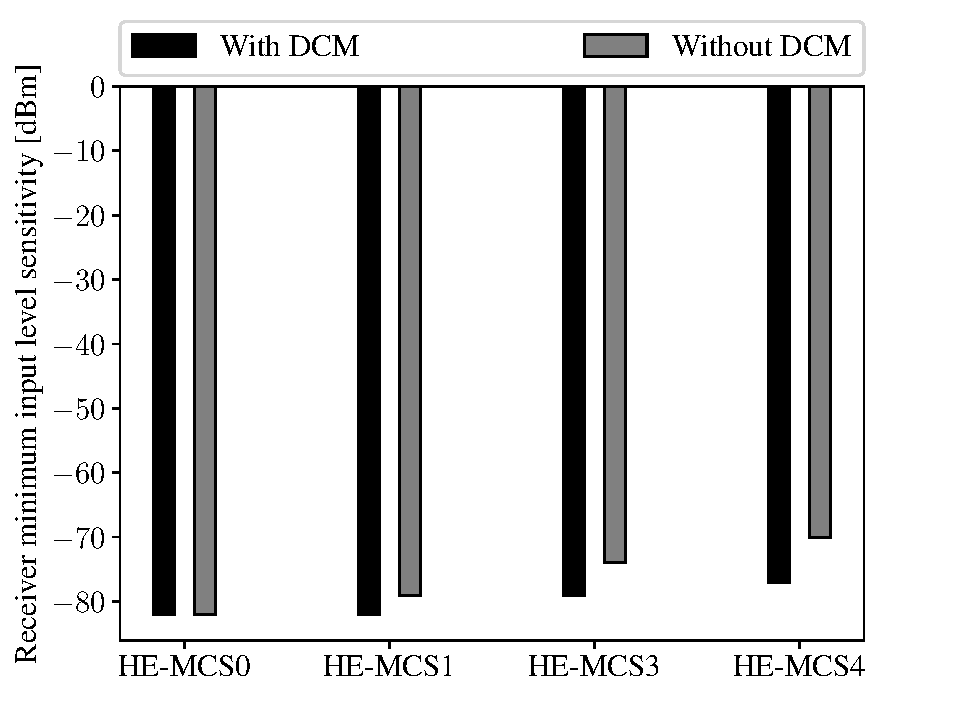
\includegraphics[width=0.95\textwidth]{figures/Receiver_minimum_DCM.pdf}
	\caption{Receiver minimum input level sensitivity for different HE-MCS values according to \cite{noauthor_ieee_2021}, where \ac{PER} is less than \SI{10}{\percent}}%
	\label{fig:ReceiverSensitivityDCM}%
\end{figure}

A similar development of the receiver minimum input sensitivity can also be observed for higher \ac{BW}, except that the lowest value increases with \ac{BW}.

The higher probability of achieving data is achieve at the expense of the data rate. The same amount of data now takes twice as long to transmit. 

\cite{noauthor_ieee_2021} lists the theoretically possible data rates. These reveal that the maximum achievable data rate with DCM is only half of the achievable data rate without DCM.

Support for \ac{DCM} is only optional in the IEEE 802.11ax standard and can only be used for HE-\ac{MCS}-\num{0}, HE-\ac{MCS}-\num{1}, HE-\ac{MCS}-\num{3} and HE-\ac{MCS}-\num{4} for \numrange{1}{2} spatial transmission streams \cite{noauthor_ieee_2021}.

\textcite{jacob_system-level_2020} and \textcite{triwinarko_phy_2021} mention plans, to allow using \ac{DCM} in the physical layer of IEEE 802.11bd.

BER Ryu


\begin{comment}
	Allowed relative constellation error versus constellation size RMS error over subcarriers and Frequency
	
	Table 27-51—Receiver minimum input level sensitivity
	
	Table 27-52—Minimum required adjacent and nonadjacent channel rejection levels
	optional feature \cite{noauthor_ieee_2021}
	
	HE SU PPDU HE ER SU PPDU not for GI 800 ns \cite{noauthor_ieee_2021}
\end{comment}


\subsubsection*{Extended Range}
Since IEEE 802.11ax the Extended Range Mode exists, which defines the new HE ER SU \ac{PPDU} as physical layer amendment \cite{noauthor_ieee_2021} \cite{afaqui_ieee_2017}.
\textcite{deng_ieee_2017} explains that the HE ER SU \ac{PPDU} format is intended to extend the range of a single station to access point transmission. This is accomplished, according to the authors, by the PPDU containing a repetition of the HE-SIG-A field.

In addition, the authors explain that preamble is power-boosted, which is limited to \SI{3}{\decibel} in \cite{noauthor_ieee_2021} \cite{jacob_system-level_2020}, to guarantee reliable transmission for longer ranges.

The IEEE 802.11ax \cite{noauthor_ieee_2021} standard defines that the HE ER SU \ac{PPDU} format may only be used when 20 Mhz transmissions with either 242 RU with HE-MCS-0 - HE-MCS-2 or 106 RU with HE-MCS-0 are used on a spatial stream. In addition, one can use \ac{DCM}.

Optionally, the HE ER SU \ac{PPDU} may also be transmitted with a \ac{GI} of \SI{800}{\nano\second}, where an additional application of \ac{DCM} is forbidden. 
	
\textcite{jacob_system-level_2020} and \textcite{triwinarko} add, that it is planned to use the extended range mode also in the IEEE 802.11bd standard.

\subsubsection*{\acf{MIMO}}
In order to further exploit the physical layer capabilities, the single transmitting and receiving antenna systems called Single-Input-Single-Output can be extended to \ac{MIMO} - systems.
\textcite{sauter_wireless_2022} describe the idea behind \ac{MIMO} as the usage of multiple transmit antennas and multiple receiving antenna. Spatial multiplexing is used so that the transmitted signals from each antenna are reflected differently on objects and can thus be received from different directions at the receiver antennas. 

The authors explain that since IEEE 802.11n it is possible to use up to four MIMO streams. This number was increased again to up to eight MIMO streams in IEEE 802.11ax \cite{noauthor_ieee_2021}. Since data can be sent simultaneously via each MIMO stream, the theoretical data rate can thus increase proportionally depending on the usable streams.
\begin{comment}
SU-MIMO, MU-MIMO, UL, DL
\end{comment}

MU-\ac{MIMO} DCM only appicable, when RU contains only data for one user.
\cite{noauthor_ieee_2021} 607 not applicable with DCM
$NUM\_STS$ = Number of Spatial Streams
$n_{ss}$ = $NUM\_STS / (1 + STBC)$
\subsubsection*{\acf{STBC}}
\textcite{abbas_efficient_2016} sagt zudem, dass \ac{MIMO} spatial streams dazu genutzt werden kann, um die Qualität des empfangenen Signals zu verstärken.
Das geschieht durch \ac{STBC}. Dabei werden den Autoren nach redundant copies of data transmitted via different antenna to the receiver. At the receiver the received data copies are combined and a maximum likelihood detector is applied in order to retain a high quality signal \cite{santumon_space-time_2012}.
\ac{STBC} is a technique used in Wi-Fi networks to improve the reliability and robustness of wireless communications.
\ac{STBC} encodes multiple redundant copies of data at the transmit side, which are transmitted in different spatial streams to
reduce the effects of fading and interference. At the receiver side, these multiple copies are combined to improve the
signal quality and decrease the \ac{PER}.

Thes results  in \ac{STBC} improving the reliability and robustness of wireless communications.
Here, \textcite{stamoulis_impact_2003} has investigated the potential effect of \ac{STBC} on Wi-Fi. Their simulations showed that\ac{STBC} can increase the range and robustness for IEEE 802.11a.
In addition, the authors concluded  that \ac{STBC} increases the \ac{SNR} in nearly all cases at the same throughput or even allows higher \ac{MCS} values to be used,
thus allowing a higher throughput at the same \ac{SNR}.

\textcite{ghosh_error_2014} analyzed the error rate performance for increasing number of used antenna and found out, that a lower bit error rate can be achieved
when increasing the number of transmit antennas with \ac{STBC}.

\textcite{gast_80211n_nodate} and \textcite{sauter_wireless_2022} mention, that \ac{STBC} can extend the signal range due to the increased robustness.

IEEE 802.11ax stations can optionally use \ac{STBC} the following conditions \cite{noauthor_ieee_2021}:
\begin{itemize}
	\item DCM is not applied
	\item The number of spatial streams is \num{2}
	\item The \ac{GI} is not \SI{0.8}{\nano\second} and the symbol length is not \SI{12.8}{\micro\second}
\end{itemize}




\cite{gast_80211n_nodate} states, that \ac{STBC} is only supported in one fifth of the Wi-Fi CERTIFIED devices.
Group addressed frames


HE Capabilities nur so gut, wie das schlechteste Glied